\chapter{Introduction}
\label{chap:chap1}

Nuclear-polarized noble gases have been proven to be very useful in various applications, such as polarized targets for electron scattering experiments~\cite{PhysRevLett.71.959}, magnetic resonance imaging~\cite{MRI} and neutron scattering experiments~\cite{Neutron}. Polarized $^3$He has been particularly useful for studying spin-dependent interactions involving neutrons because, to first-order approximation, a $^{3}$He nucleus has a pair of protons with paired spins and a single neutron that carries most of the nuclear spin. Free neutrons are not used as targets because they decay with a lifetime of about 14 minutes, 42 seconds. 

\section{Motivation and Approved JLab Experiments}

The neutron electromagnetic form factors, $G_E^n$ and $G_M^n$ play essential roles for understanding nucleon structure. At non-relativistic energies, they are the Fourier transforms of the electric charge and magnetic moment distributions. Even at relativistic energies, the elastic form factors provide unique information on the transverse structure of the nucleon~\cite{PhysRevLett.99.112001, PhysRevLett.100.032004}. Double-polarization experiments on the proton showed that the ratio of the proton's electric and magnetic elastic form factors, $G_E^p/G_M^p$, declines nearly linearly as the four momentum transfer squared, $Q^2$, increases, in sharp contrast to expectations~\cite{PhysRevLett.84.1398}. These measurements caused a resurgence of interest in nucleon structure, and shed light on the importance of quark orbital angular momentum. More recent double-polarization experiments measured the neutron electric form factor $G_E^n$ up to a $Q^2$ of $\rm 3.4\,GeV^2$ (E02-013)~\cite{Phys.Rev.Lett.105.262302}, and showed behavior that was generally consistent with models that described well the earlier proton results. The neutron results, when combined with the proton results, also made it possible to extract the form factors for the individual up- and down-quark flavors~\cite{PhysRevLett.106.252003}. Significantly different $Q^2$ dependence was seen for the up- and down-quarks, a difference that some theorists have interpreted as evidence for the importance of diquark correlations.  

The multiple surprises that have emerged from the study of nucleon elastic form factors at Jefferson Laboratory (JLab) have underscored the value of performing such studies at high values of $Q^2$. For the neutron, predictions for the behavior of the ratio of the electric and magnetic elastic form factors, $G_E^n/G_M^n$, vary significantly from one model or calculation to another. A particularly compelling example, based on the Dyson-Schwinger Equation (DSE) formalism, predicts a dramatic turnover and zero crossing in the vicinity of $Q^2 = \rm 10\,GeV^2$~\cite{Cloet}. The verification of this prediction would have profound impact on our understanding of nucleon structure. An important part of the future program at JLab to explore the high-$Q^2$ behavior of the elastic nucleon form factors is the Super Bigbite Spectrometer (SBS) program. The SBS experiment to measure $G_E^n/G_M^n$ up to $Q^2 = \rm 10\,GeV^2$, E12-09-016, is a major motivating factor for the work described in this thesis. The count rate associated with the elastic form factors drops off very quickly with increasing $Q^2$. This in turn puts pressure on all aspects of the experiment to achieve adequate statistics, including running the polarized $^3$He target at high luminosity.  

Another important issue in understanding nucleon structure is the spin structure associated with the quarks. Polarized deep inelastic scattering provides a window into the spin carried by the quarks, and a particularly useful observable is the spin asymmetry $A_1^n$, that describes the spin dependence of the virtual photo absorption cross section. It is particularly useful to measure $A_1^n$ at high values of Bjorken $x$, where several predictions exist. Both constituent quark models and perturbative QCD predict that $A_1^n \rightarrow 1$ as $x_{\rm Bj} \rightarrow 1$, but it is also the case that count rates drop quickly toward high values of  $x_{\rm Bj}$. Two experiments are currently approved at JLab that will measure $A_1^n$ up values of  $x_{\rm Bj}$ in excess of 0.7; they are E12-06-122 in Hall A, and E12-06-110 in Hall C. Both of these experiments will require a polarized $^3$He target capable of running at high luminosity and thus depend critically on the work describe here.  

\section{Overview of Recent Target Development}

An early use of polarized $^3$He targets in electron scattering experiments was at the Stanford Linear Accelerator Center (SLAC) in the year of 1992. The experiment was known as E142 and investigated the spin structure of neutrons~\cite{PhysRevLett.71.959}. Recent experiments were conducted at Jefferson Laboratory (JLAB) in Newport News, Virginia, such as the aforementioned E02-013, also known as ``Measurement of the Neutron Electric Form Factor $G^n_E$ at High $Q^2$ ". Other experiments involved the investigation of single-spin asymmetries in semi-inclusive deep inelastic scattering~\cite{PhysRevLett.107.072003}.

The $^3$He targets used in these experiments were polarized with the technique of Spin-Exchange Optical Pumping (SEOP). Fig.~\ref{TargetCell} shows schematically a typical target, also referred to as a ``target cell". These cells were made of GE180 glass and used a two-chambered design. The top chamber, known as the “pumping chamber”, is where $^{3}$He is polarized through SEOP. The bottom chamber, known as the “target chamber”, is where electron scattering occurs. The two ends of the target chamber where electron beam enters and exits are known as the ``end windows". Great effort has been made in our lab to develop this generation of cells. Alkali-hybrid SEOP together with narrowband laser-diode arrays have increased the $^{3}$He polarization from 37\% to 70\%. Among other things, we also carefully studied an additional spin relaxation mechanism that limits the maximum achievable $^{3}$He polarization, which can be characterized by something referred to as the ``X Factor"~\cite{PhysRevLett.96.083003}. Analysis of data accumulated through developing this generation of target cells were thoroughly discussed in Ref.~\cite{PhysRevC.91.055205}, part of which will be presented in chapter 4. 

\begin{figure}[H]
	\centering
	\resizebox{0.91\textwidth}{!}{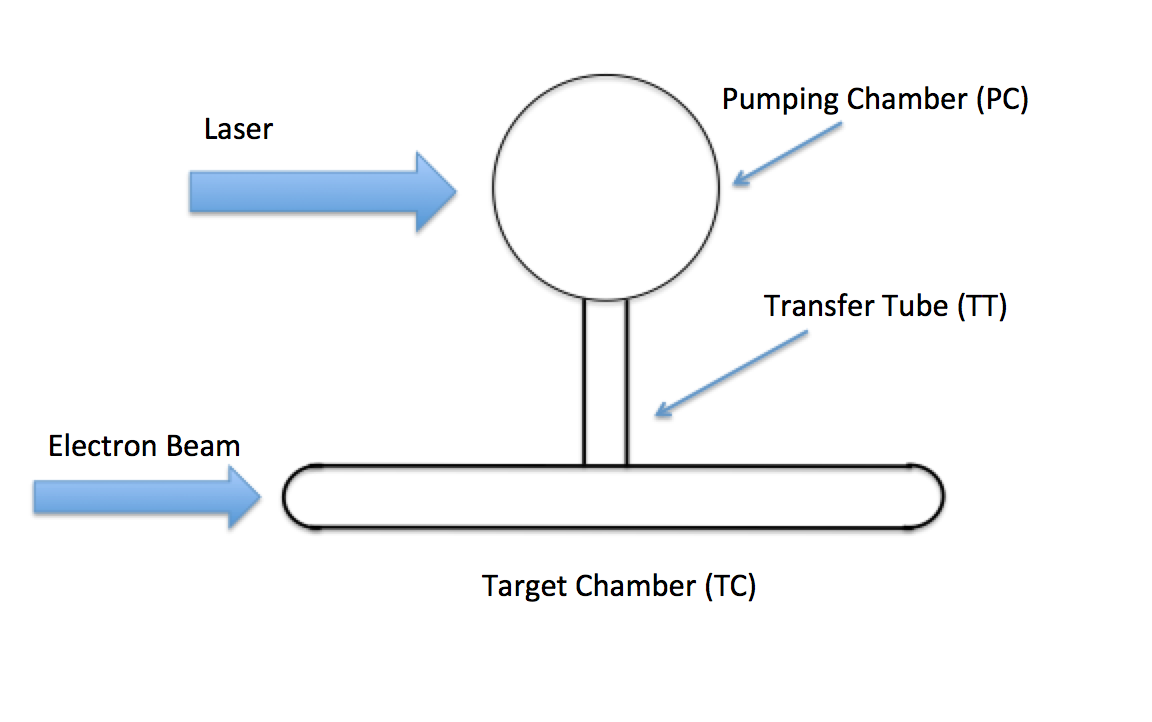
\includegraphics{TargetCell.png}}
	\caption{{ A schematic representation of a target cell. The dimensions of different parts of the cell are not to scale.}}
	\label{TargetCell}
\end{figure}

\section{New Generation Target Cells}

The future experiments planned for the JLab 12GeV era after the energy upgrade will be much more demanding in terms of target cell performance. In particular, there is a desire to run experiments with higher luminosity, where luminosity is the product of gas density in the target, interaction length and beam current. Increased luminosity will lead to more interactions that depolarize the target. We have designed and tested a new style cell that utilizes convection instead of diffusion to increase the rate at which the polarization in the target chamber is replenished by polarized gas from pumping chamber~\cite{PhysRevC.84.065201}. We have obtained over 50\% polarization with controllable convection speed so far.

An additional problem that comes with higher beam current is that the glass end windows of traditional design are not likely to survive the experiments. Our group started exploring the option of using metal end windows eight years ago. Fig~\ref{metal_end_windows} shows an example configuration of such a target. The first problem to solve is to find out the correct material and the proper technique to incorporate metal without introducing significant spin relaxation while still being able to hold high pressure gas (12 atm) inside. This is a brand new technique that may have a profound impact on future cell designs once fully developed. Although no metal end windows have been tested so far, through carefully examining multiple glass cells with different kinds metal tubes (much larger in area compared to the end windows that will be used in JLAB experiments) attached, we have developed a reliable way of incorporating metal into target cells without introducing excessive spin relaxation. We believe the next generation target cells used in the 12GeV era will be able to utilize metal end windows. In our test cells, the metals tubes were connected to Pyrex glass with Houskeeper seals~\cite{Houskeeper} and stayed intact through high pressure tests. After exploring options such as pure copper, gold coated copper, titanium, stainless steel, gold coated titanium, we have established that electroplating gold on a copper substrate yields the best result so far. We have achieved a 15.6 h relaxation time with a Pyrex cell that had a 5'' long by 1'' diameter gold coated copper tube attached horizontally. The additional relaxation rate introduced by the metal surface is proportional to the area of the gold surface. By comparing relaxation rates of test glass-and-metal cells with pure-glass control cells, the relaxation rate due to the gold surface was extracted. With this result, we believe the relaxation rate introduced by small metal windows in a target will be less than 1/93.06 hr$^{-1}$. To the best of our knowledge, our group was the first to have proved the potential of incorporating metal into target cells in the presence of alkali vapor. 

\begin{figure}[t!]\label{metal_end_windows}
	\centering
	\resizebox{0.91\textwidth}{!}{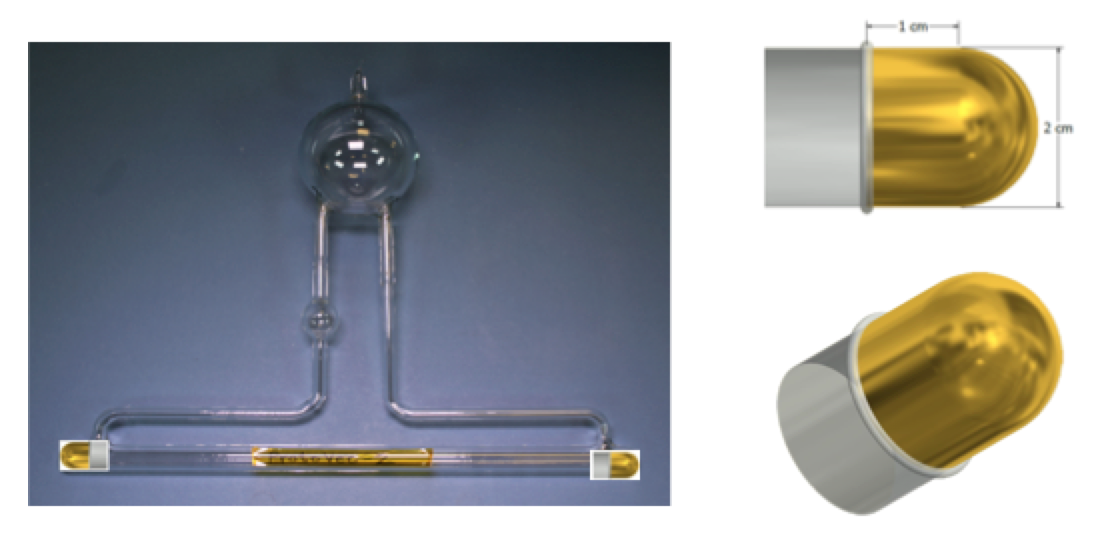
\includegraphics{metal_end_windows.png}}
	\caption{{A diagram of convection style target cell with metal end windows. }}
	\label{metal_end_windows}
\end{figure}

\section{Structure of This Thesis}

This thesis focuses on both a discussion of the development of high-performance polarized $^3$He targets that utilize spin-exchange optical pumping (SEOP) and the development of future target cells that incorporate metal end windows. Chapter 2 gives a general description of SEOP. Chapter 3 introduces polarimetry techniques used in our lab for target cell characterization. Chapter 4 discusses the results collected in our lab from over a decade of development of $^3$He target cells, in which the spin-exchange rate constant for K and $^3$He is calculated and the so-called ``X Factor" is studied. Chapter 5 presents the development process of target cells with metal parts that aims to incorporate metal end windows into future cells for the JLab 12 GeV era experiments. Chapter 6 presents some conclusions and discusses the implications for future work.













